%requis
\documentclass[a4paper,11pt]{report}
\usepackage[utf8x]{inputenc}
\usepackage[T1]{fontenc}
\usepackage[frenchb]{babel}
\usepackage{graphicx}
\usepackage{array}
\usepackage{fancyhdr}
\usepackage{listings}
\pagestyle{fancy}
\usepackage{color}

\definecolor{javared}{rgb}{0.6,0,0} % for strings
\definecolor{javagreen}{rgb}{0.25,0.5,0.35} % comments
\definecolor{javapurple}{rgb}{0.5,0,0.35} % keywords
\definecolor{javadocblue}{rgb}{0.25,0.35,0.75}  
\definecolor{backgrnd}{gray}{0.9}
 
\lstset{ %
  language=Octave,                % the language of the code
  basicstyle=\footnotesize,           % the size of the fonts that are used for the code
  numbers=left,                   % where to put the line-numbers
  numberstyle=\tiny\color{black},  % the style that is used for the line-numbers
  stepnumber=2,                   % the step between two line-numbers. If it's 1, each line 
                                  % will be numbered
  numbersep=5pt,                  % how far the line-numbers are from the code
  backgroundcolor=\color{white},      % choose the background color. You must add \usepackage{color}
  showspaces=false,               % show spaces adding particular underscores
  showstringspaces=false,         % underline spaces within strings
  showtabs=false,                 % show tabs within strings adding particular underscores
  frame=single,                   % adds a frame around the code
  rulecolor=\color{black},        % if not set, the frame-color may be changed on line-breaks within not-black text (e.g. commens (green here))
  tabsize=2,                      % sets default tabsize to 2 spaces
  captionpos=b,                   % sets the caption-position to bottom
  breaklines=true,                % sets automatic line breaking
  breakatwhitespace=false,        % sets if automatic breaks should only happen at whitespace
  title=\lstname,                   % show the filename of files included with \lstinputlisting;
                                  % also try caption instead of title
  keywordstyle=\color{javapurple},          % keyword style
  commentstyle=\color{javagreen},       % comment style
  stringstyle=\color{javared},         % string literal style
  escapeinside={\%*}{*)},            % if you want to add a comment within your code
  morekeywords={*,...},               % if you want to add more keywords to the set
  morecomment=[s][\color{javadocblue}]{/**}{*/}
}
% premiere Page
\title{\Huge \textbf{\fontfamily{phv}Projet tutoré \\
Outils de gestion centralisée de machines virtuelles}}
\author{Bocca Augustin,Lamouroux Mathieu,Michaux Sebastien,Tournois Julien}
\date{vendredi 17 février}

\begin{document}

%formattage de l'entete
\renewcommand{\chaptermark}[1]{\markboth{#1}{}} \renewcommand{\sectionmark}[1]{\markright{#1}}
\renewcommand{\headrulewidth}{0.25mm}
\lfoot{\center Outils de gestion centralisée de machines virtuelles}
\renewcommand{\footrulewidth}{0.25mm}
%titre
\maketitle

\textbf{Préambule:}
\tableofcontents
  \chapter{Introduction}
    \section{Présentation de Grid5000}

Aujourd’hui, grâce à Internet, il est possible
d’interconnecter des machines du monde entier pour
traiter et stocker des masses de données. Cette collection
hétérogène et distribuée de ressources de stockage et de
calcul a donné naissance à un nouveau concept : les
grilles informatiques. L’idée de mutualiser les ressources
informatiques vient de plusieurs facteurs, évolution de la
recherche en parallélisme qui, après avoir étudié les
machines homogènes, s’est attaquée aux environnements
hétérogènes puis distribués ; besoins croissants des
applications qui nécessitent l’utilisation toujours plus
importante de moyens informatiques forcément répartis.
La notion de grille peut avoir plusieurs sens suivant le
contexte : grappes de grappes, environnements de type
GridRPC (appel de procédure à distance sur une grille).,
réseaux pair-à-pair, systèmes de calcul sur Internet, etc...
Il s’agit d’une manière générale de systèmes dynamiques,
hétérogènes et distribués à large échelle. Un grand
nombre de problématiques de recherche sont soulevées
par les grilles informatiques. Elles touchent plusieurs
domaines
de l’informatique :algorithmique,
programmation, intergiciels, applications, réseaux.
L’objectif de GRID’5000 est de construire un instrument
pour réaliser des expériences en informatique dans le
domaine des systèmes distribués à grande échelle (GRID).
Cette plate-forme, ouverte depuis 2006 aux chercheurs de
la communauté grille, regroupe un certain nombre de sites
répartis sur le territoire national. Chaque site héberge une
ou plusieurs grappes de processeurs. Ces grappes sont
alors interconnectées via une infrastructure réseau dédiée
à 10 Gb/s fournie par RENATER. À ce jour, GRID’5000
est composé de 9 sites: Lille, Rennes, Orsay, Nancy,
Bordeaux, Lyon, Grenoble, Toulouse et Nice. Début 2007,
GRID’5000 regroupait plus de 2500 processeurs et près
de 3500 cœurs.

\newpage
\begin{center}

\includegraphics{g5k.png}
\underline{\textit{Architecture Grid5000}}
\end{center}

  \subsection{Infrastructure des sites}
Chaque site héberge :
\begin{itemize}
\item un frontend, serveur permettant d'accéder aux clusters disponibles ,
\item un serveur de données, pour centraliser les données utilisateurs ,
\item plusieurs clusters, c'est-à-dire des grappes de machines homogènes, appelées noeuds (nodes).
\end{itemize}
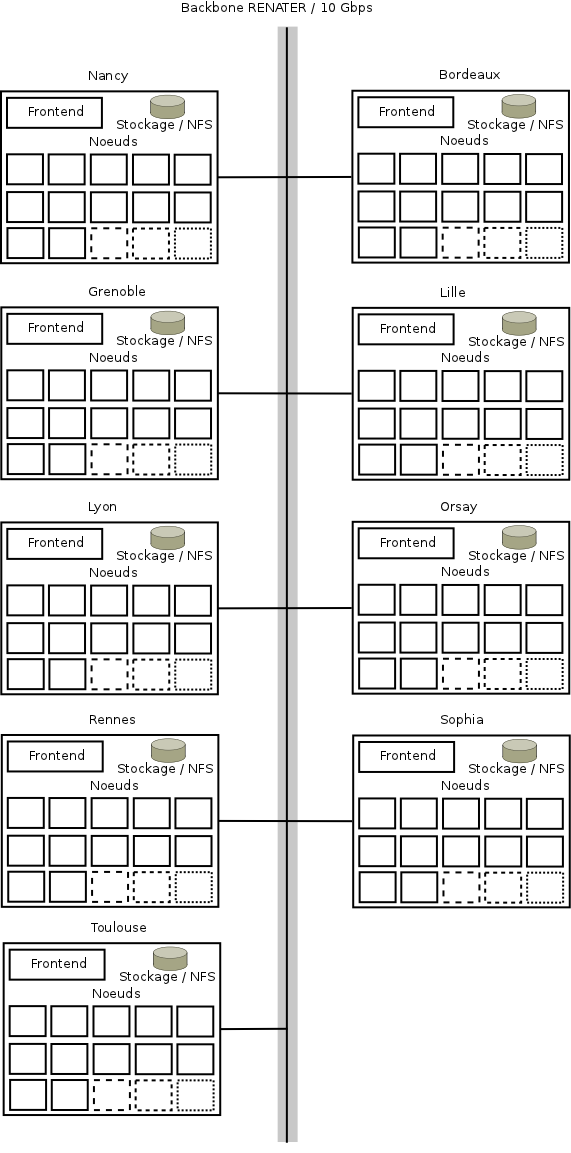
\includegraphics[width=10cm,height=15cm]{g5k1.png}
L'utilisateur de Grid 5000 accède à chaque site par son frontend en utilisant le protocole SSH.\\
Commande:
\begin{lstlisting}
ssh jdoe@access.grid5000.fr
\end{lstlisting}
Sur tous les serveurs du site, un répertoire home, local à chaque site, est monté avec NFS 2 .
A partir du frontend, il est possible d'accéder aux machines des clusters en exectuant des réservations à l'aide de la commande:
\begin{lstlisting}
oarsub
\end{lstlisting}
Gràce à notre tuteur, M. Lucas Nussbaum nous avons pu visiter la salle serveurs du site de Nancy située au Loria, 
ainsi qu'une présentation de la plate-forme (matériel utilisé, connexions réseau,
administration).
\quotation\textit{Une description détaillée du site de Nancy est disponible sur le site de Grid 5000.}

  \subsection{Réseau}
Les sites et toutes les machines qu'ils comprennent sont interconnectés par RENATER 3 en 10Gbits/s. De
plus, chaque site peut disposer de plusieurs réseaux locaux 4 :
\begin{itemize}
\item réseau en ethernet, 1 Gb/s
\item réseaux hautes performances (Infiniband 20 Gb/s ou 10 Gb/s, et Myrinet 20 Gb/s)
\end{itemize}

  \subsection{Environnement logiciel}
Tous les serveurs de Grid 5000 fonctionnent sous Debian GNU/Linux.
A partir du frontend, l'utilisateur peut réserver des machines en utilisant la suite de logiciels OAR dédiée à
la gestion de ressources de clusters, et déployer ses propres images de systèmes à l'aide des outils kadeploy.
Il y a deux types de réservation :
\begin{itemize}
\item par défaut, pour des besoins de calcul avec OpenMPI ;
\item pour le déploiement d'environnements (deploy ).
\end{itemize}

     \newpage
     \section{Présentation du projet}
     \paragraph{Objectif}
Mettre en place, évaluer et comparer différents outils permettant de gérer de manière
centralisée et automatisée une infrastructure basée sur des machines virtuelles: Ganeti,
OpenXenManager, virt-manager, Archipel...
      \section{Introduction à la virtualisation}

    \chapter{Ganeti}
      \section{Introduction}
Ganeti est un outil de gestion de machines virtuelles se basant sur les technologies de virtualisation existantes comme XEN et KVM.\\
Ganeti nécessite un logiciel de virtualisation pré-installé sur les serveurs afin de pouvoir fonctionner. Une fois installé, 
l'outil prendra en charge la partie gestion des instances virtuelles (Xen DomU), par exemple, la gestion de création de disque, 
l'installation du système d'exploitation (en coopération avec les scripts d'installation du système d'exploitation 
spécifique), et le démarrage, l'arrêt, le basculement entre les systèmes physiques. Il a été conçu pour faciliter la gestion de 
cluster de serveurs virtuels et de fournir une récupération rapide et simple.
      \section{Installation}
\begin{lstlisting}
apt-get install ganeti2 ganeti-htools ganeti-instance-debootstrap
\end{lstlisting}
Puis dans /etc/host il faut ajouter l'adresse IP du node avec le nom de l'host ainsi que l'adresse du cluster :\\
\begin{lstlisting}
10.144.64.1 cluster1
172.16.65.56 griffon-56.nancy.grid5000.fr
\end{lstlisting}
\begin{quotation}
\textit{Lorsque l'on a plusieur nodes il faut une autre adresse Ip au cluster car elle doit etre accessible à tous les nodes\\}
\end{quotation}
Ensuite, dans /boot/ creer des liens symboliques :
\begin{lstlisting}
ln -s vmlinuz-2.6.32-5-xen-amd64 vmlinuz-2.6.xenU
ln -s initrd.img-2.6.32-5-xen-amd64 initrd.img-2.6.xenU
\end{lstlisting}
Il est obligatoire de creer un LVM d'au moins 20Go sur tous les noeuds car ce volume permettra de stocker par exemple les systèmes de fichiers 
, si vous voulez utiliser toutes les fonctionnalités ganeti:\\
\begin{lstlisting}
umout /dev/sda5
pvcreate /dev/sda5
vgcreate xenvg /dev/sda5
\end{lstlisting}
Dans /ect/network/interface remplacer le paragraphe de eth0 par celle du brige xen-br0 :
\begin{lstlisting}
auto xen-br0
iface xen-br0 inet static
address 172.16.65.56 #address du node
netmask 255.255.240.0 
network 172.16.64.0
broadcast 172.16.79.255
gateway 10.144.64.254
bridge_ports eth0
bridge_stp off
bridge_fd 0ction{Utilisation}
\end{lstlisting}
\paragraph{\textbf{Pourquoi un nom d'hôte?} }
Bien que la plupart des distributions utilisent uniquement 
le nom court dans le fichier / etc / hostname, ganeti utilise le nom 
complet. La raison en est que 'le nom d'hôte-fqdn' appel la bibliothèque de résolution. Deplus ganeti peut être utilisé entre 
autres pour accueillir les serveurs DNS.

\section{Utilisation de ganeti}
Initialiser le cluster avec ganeti :
\begin{lstlisting}
gnt-custer init --no-drbd-storage cluster1
\end{lstlisting}
ajouter le node :
\begin{lstlisting}
gnt-node add griffon-56.nancy.grid5000.fr
\end{lstlisting}

Il est ensuite possible de verifier la liste des nodes avec :
\begin{lstlisting}
gnt-node list
\end{lstlisting}
Qui devrait renvoyer quelque chose comme cela :\\
%\begin{lstlisting}
Node                         DTotal  DFree MTotal MNode MFree Pinst Sinst\\
griffon-56.nancy.grid5000.fr 283.2G 283.2G  
%\end{lstlisting}  
    
  \newpage
    \chapter{Scripts}
      \section{réservation}
      \begin{lstlisting}
puts "-----------------------------------------"
puts "Souhaitez vous reserver des noeuds?(y/n)"
loop do
  test = gets.chomp
  if test.eql?("n")
    puts "#####################"
    puts "#sortie du programme#"
    puts "#####################"
    break;
  end
  if test.eql?("y")
    #Reservation de machines                                                 
    puts "---------Script de reservation-----------"
    puts "Choisir un nombre de noeud:"
    noeuds = gets.chomp.to_i
    puts "Choisir un temps de reservation(HH:MM:SS):"
    temps = gets
    puts "\nVous avez reserve #{noeuds} noeuds 
	  pour une duree de #{temps}"
    puts "-----------------------------------------"
    exec "oarsub -I -t deploy -n'virtu' -l 
	  slash_22=1+nodes=#{noeuds},walltime=#{temps}"
    break;
  end
end
      \end{lstlisting}
      
      \newpage
      \section{déploiment}
      \begin{lstlisting}
#Deployer une image cree
puts "Voulez vous deployer une image?(y/n)"
loop do
  test = gets.chomp
  if test.eql?("n")
    puts "#####################"
    puts "#sortie du programme#"
    puts "#####################"
    break;
  end
  if test.eql?("y")
    #choix de l'image                                                                                                                 
    puts "-----------------------------------------------"
    puts "image disponibles:"
    puts `ls /home/$USER/image | grep .env`
    puts "-----------------------------------------------"
    puts "Choix de la distibution(tout saisir):"
    debian = gets.chomp
    puts "-----------------------------------------------"
    exec"kadeploy3 -f $OAR_FILE_NODES -a #{debian} -k 
	$HOME/.ssh/id_rsa.pub"
    break;
  end
end
#Deploiment de l environement sur les noeuds reserves                          
puts "Voulez vous deployer un environement?(y/n)"
loop do
  test = gets.chomp
  if test.eql?("n")
    puts "#####################"
    puts "#sortie du programme#"
    puts "#####################"
    break;
  end
  if test.eql?("y")                                                            
    #choix de la version a deployer                                            
    puts "-----------------------------------------------"
    puts "distributions disponibles:"
    puts `kaenv3 -l | cut -d - -f1 | uniq | tail -n +3`
    puts "-----------------------------------------------"
    puts "Choix de la distibution:"
    debian = gets.chomp
    puts "-----------------------------------------------"
    puts "version de la distribution:"
    puts `kaenv3 -l | grep #{debian}| cut -d ' ' -f1`
    debian = debian+"-x64-"
    puts "-----------------------------------------------"
    puts "Choix de la version de la distribution a deployee 
	  (sans #{debian}):"
    version = gets.chomp
    version = debian+version
    puts version
    exec"kadeploy3 -e #{version} -f $OAR_FILE_NODES -k 
	$HOME/.ssh/id_rsa.pub"
    break;
  end
end
      \end{lstlisting}

      
      \section{configuration de base}
      \begin{lstlisting}
########################################################
#------------------Configuration minimale--------------#
#______________________________________________________#

#recuperation des noeuds reserves
cat $OAR_FILE_NODES | uniq  > $HOME/script_base/list_nodes
list_nodes="$HOME/script_base/list_nodes"

echo "-----------------------------------"
echo "Liste des machines reservee:"
cat $list_nodes
echo "-----------------------------------"
echo "Copie des clees SSH vers toutes les machines."
for node in $(cat $list_nodes)
do
	scp $HOME/.ssh/id_rsa* root@$node:~/.ssh/
done
echo "-----------------------------------"

#mise a jour des noyaux
taktuk -l root -f $list_nodes broadcast exec [ apt-get update ]
taktuk -l root -f $list_nodes broadcast exec [ apt-get dist-upgrade 
      -q -y --force-yes ]
#changement des mdp root
taktuk -l root -f $list_nodes broadcast exec [ 'echo -e 
      pttvirtu\npttvirtu" | passwd root' ]
      \end{lstlisting}

      \newpage
      \section{installation de ganeti}
\begin{lstlisting}
#!/bin/bash
#passage en wheezy
rm /etc/apt/sources.list
echo "## wheezy security" > /etc/apt/sources.list
echo "deb http://security.debian.org/ wheezy/updates main contrib non-free" >> /etc/apt/sources.list
echo "deb-src http://security.debian.org/ wheezy/updates main contrib non-free" >> /etc/apt/sources.list
echo " " >> /etc/apt/sources.list
echo "#wheezy" >> /etc/apt/sources.list
echo "deb http://ftp.fr.debian.org/debian/ wheezy main contrib non-free" >> /etc/apt/sources.list
echo "deb-src http://ftp.fr.debian.org/debian/ wheezy main contrib non-free" >> /etc/apt/sources.list
#Installation de ganeti 
apt-get update
apt-get dist-upgrade -y --force-yes
apt-get install -y --force-yes ganeti2 ganeti-htools ganeti-instance-debootstrap
echo "Ajout du node dans /etc/hosts"
hostname=`cat /etc/hostname`
#recuperation des variables
#ip du node
ifconfig eth0 > troll
ipnode=`head -2 troll | tail -1 | cut -d':' -f2 | cut -d' ' -f1`
echo $ipnode $hostname >> /etc/hosts
#ip du broadcast
ipbroadcast=`head -2 troll | tail -1 | cut -d'B' -f2 | cut -d':' -f2 | cut -d' ' -f1`
#ip du masque de sous reseau
ipmask=`head -2 troll | tail -1 | cut -d'M' -f2 | cut -d':' -f2 | cut -d' ' -f1`
#ip du reseau
ipnetwork=`head -1 ipnetwork`
#ip de la passerelle
ipgateway=`head -1 ipgateway`
#ajout de cluster1 dans dans /etc/hosts
echo "ajout de cluster1 dans /etc/hosts"
ipcluster=`cat ipcluster`
echo $ipcluster "cluster1" >> /etc/hosts
#Dans /boot/ creer des liens symboliques :
ln -s /boot/vmlinuz-2.6.32-5-xen-amd64 /boot/vmlinuz-2.6.xenU
ln -s /boot/initrd.img-2.6.32-5-xen-amd64 /boot/initrd.img-2.6.xenU
#Pour le moment changera surement.
echo "creation du LVM"
umount /dev/sda5
pvcreate /dev/sda5
vgcreate xenvg /dev/sda5
#Creation du bridge xen-br0
echo " " >> /etc/network/interfaces
echo "auto xen-br0"  >> /etc/network/interfaces
echo "iface xen-br0 inet static" >> /etc/network/interfaces 
echo "address" $ipnode >> /etc/network/interfaces
echo "netmask " $ipmask >> /etc/network/interfaces
echo "network" $ipnetwork >> /etc/network/interfaces
echo "gateway"  $ipgateway >> /etc/network/interfaces
echo "broadcast" $ipbroadcast>> /etc/network/interfaces
echo "bridge_ports eth0" >> /etc/network/interfaces
echo "bridge_stp off" >> /etc/network/interfaces
echo "bridge_fd 0" >> /etc/network/interfaces
#Suppression des ligne de eth0
sed -i '9d' /etc/network/interfaces
sed -i '9d' /etc/network/interfaces
#supression des fichier temporaires
rm troll ipcluster  ipgateway  ipnetwork
#initialisation du cluster
gnt-cluster init --no-drbd-storage cluster1
#ajouter le node 
gnt-node add $hostname
#et verifier
gnt-node list
\end{lstlisting}
\end{document}          
